\documentclass[11pt,a4paper]{article}

\usepackage[utf8]{inputenc}
\usepackage[T1]{fontenc}
\usepackage[french]{babel}
\usepackage[margin=1.8cm]{geometry}
\usepackage{array}
\usepackage{longtable}
\usepackage{booktabs}
\usepackage{tabularx}
\usepackage{xcolor}
\usepackage{colortbl}
\usepackage{enumitem}
\usepackage{titlesec}
\usepackage{graphicx}
\usepackage{float}
\usepackage{amsmath}

\definecolor{titleblue}{RGB}{0,102,153}
\definecolor{lightgray}{RGB}{240,240,240}
\newcolumntype{P}[1]{>{\raggedright\arraybackslash}p{#1}}
\setlength{\parskip}{0.35em}
\setlength{\parindent}{0pt}
\renewcommand{\arraystretch}{1.25}

\titleformat{\section}{\large\bfseries\color{titleblue}}{\thesection}{0.6em}{}
\titleformat{\subsection}{\normalsize\bfseries}{\thesubsection}{0.6em}{}

\begin{document}

\begin{center}
    {\LARGE\bfseries Analyse C1 et C2 de l'API bancaire JavaScript}\\[0.25cm]
    {\large Complexité cyclomatique et graphes de flot de contrôle}\\[0.5cm]
\end{center}

\textbf{Projet :} API bancaire JavaScript\\
\textbf{Étudiant :} AMAYEN BOUSSIOM THIERRY MARTIN\\
\textbf{Matricule :} 25I2177\\
\textbf{Dépôt GitHub :} \texttt{AmayenICTL3/TPICT304}\\
\textbf{Code source analysé :} \texttt{server.js}

\section{Fonctionnalités du logiciel}

Les cinq fonctions principales étudiées à partir du code source sont :

\begin{enumerate}[leftmargin=1.2cm]
    \item créer un compte bancaire ;
    \item lister les comptes ;
    \item consulter un compte ;
    \item effectuer un dépôt ;
    \item effectuer un retrait.
\end{enumerate}

Le projet implémente aussi deux fonctions supplémentaires : l'historique des transactions et le virement entre comptes.

\section{Rappel sur C1 et C2}

\textbf{C1} : couverture des instructions. Chaque instruction doit être exécutée au moins une fois.\\
\textbf{C2} : couverture des décisions. Chaque décision doit être exercée au moins une fois à vrai et au moins une fois à faux.

\section{Complexité cyclomatique}

La complexité cyclomatique est calculée avec la forme simplifiée :

\[
M = D + 1
\]

où \(D\) est le nombre de décisions du graphe.

\begin{longtable}{|P{4.3cm}|P{2.7cm}|P{3cm}|P{5.2cm}|}
\hline
\rowcolor{lightgray}
\textbf{Fonction} & \textbf{Décisions} & \textbf{Complexité \(M\)} & \textbf{Interprétation} \\
\hline
Créer un compte & 3 & 4 & Champs obligatoires, solde négatif, dépôt initial. \\
\hline
Lister les comptes & 0 & 1 & Chemin séquentiel unique. \\
\hline
Consulter un compte & 1 & 2 & Compte trouvé ou introuvable. \\
\hline
Effectuer un dépôt & 2 & 3 & Compte introuvable, montant invalide ou dépôt valide. \\
\hline
Effectuer un retrait & 3 & 4 & Compte introuvable, montant invalide, solde insuffisant ou retrait valide. \\
\hline
\end{longtable}

\section{Graphes de flot de contrôle}

\subsection{Créer un compte}

\begin{figure}[H]
\centering
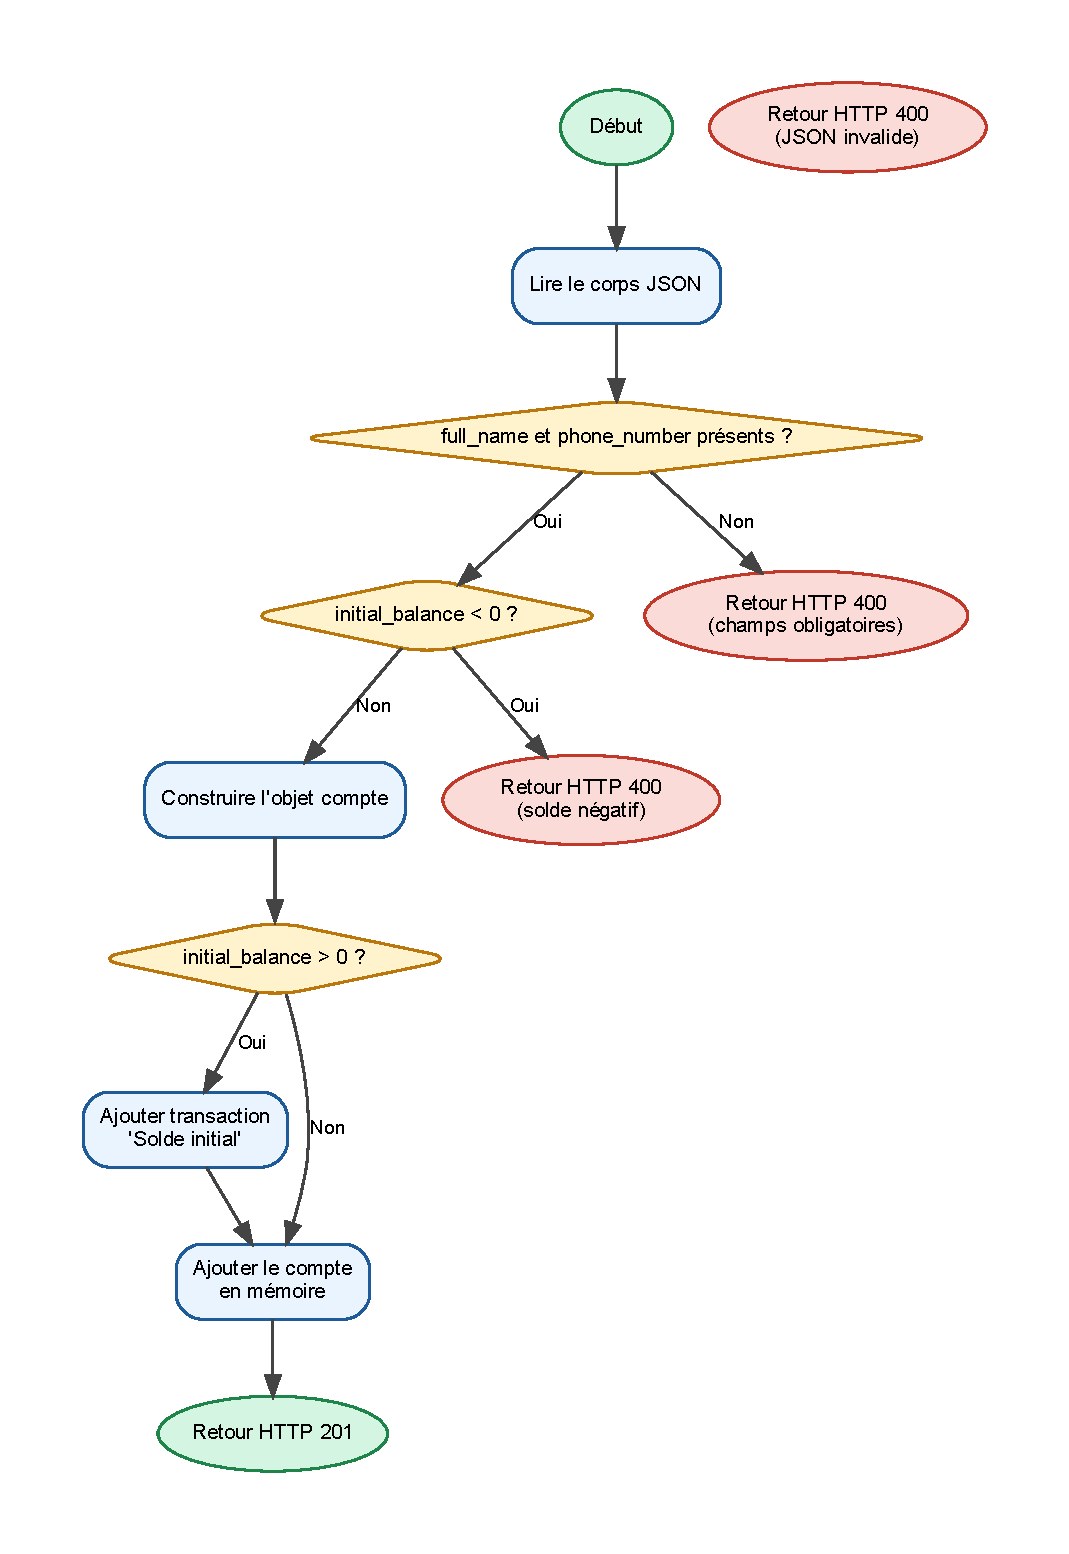
\includegraphics[width=0.78\textwidth]{docs/graphs/create_account.pdf}
\caption{Graphe de flot de contrôle de la création de compte}
\end{figure}

\textbf{Chemins principaux}
\begin{itemize}[leftmargin=1cm]
    \item P1 : champs obligatoires absents \(\rightarrow\) erreur HTTP 400.
    \item P2 : solde initial négatif \(\rightarrow\) erreur HTTP 400.
    \item P3 : création sans solde positif \(\rightarrow\) compte créé sans transaction initiale.
    \item P4 : création avec solde positif \(\rightarrow\) transaction \texttt{deposit} initiale ajoutée.
\end{itemize}

\subsection{Lister les comptes}

\begin{figure}[H]
\centering
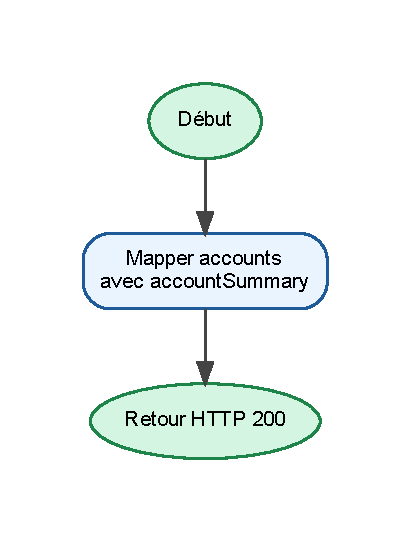
\includegraphics[width=0.45\textwidth]{docs/graphs/list_accounts.pdf}
\caption{Graphe de flot de contrôle de la liste des comptes}
\end{figure}

\textbf{Chemin principal}
\begin{itemize}[leftmargin=1cm]
    \item P1 : lecture du tableau \texttt{accounts} puis retour HTTP 200.
\end{itemize}

\subsection{Consulter un compte}

\begin{figure}[H]
\centering
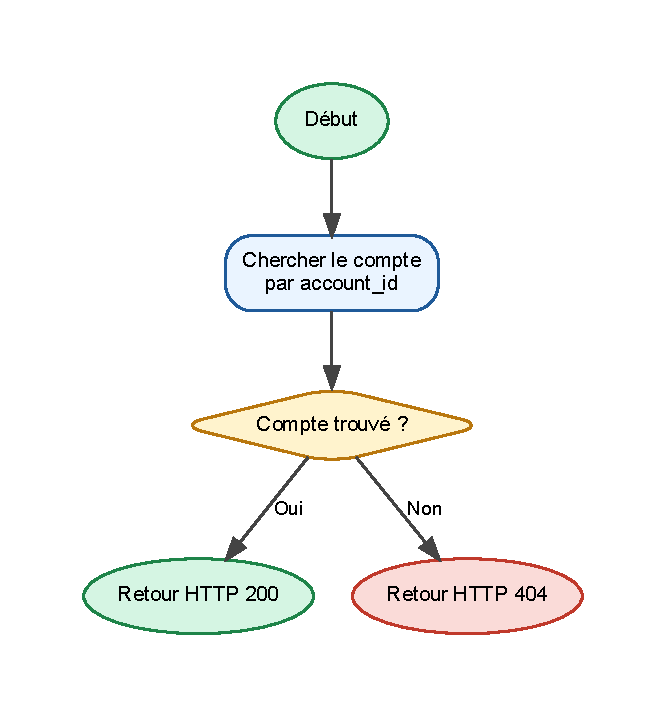
\includegraphics[width=0.55\textwidth]{docs/graphs/get_account.pdf}
\caption{Graphe de flot de contrôle de la consultation d'un compte}
\end{figure}

\textbf{Chemins principaux}
\begin{itemize}[leftmargin=1cm]
    \item P1 : compte trouvé \(\rightarrow\) retour HTTP 200.
    \item P2 : compte introuvable \(\rightarrow\) retour HTTP 404.
\end{itemize}

\subsection{Effectuer un dépôt}

\begin{figure}[H]
\centering
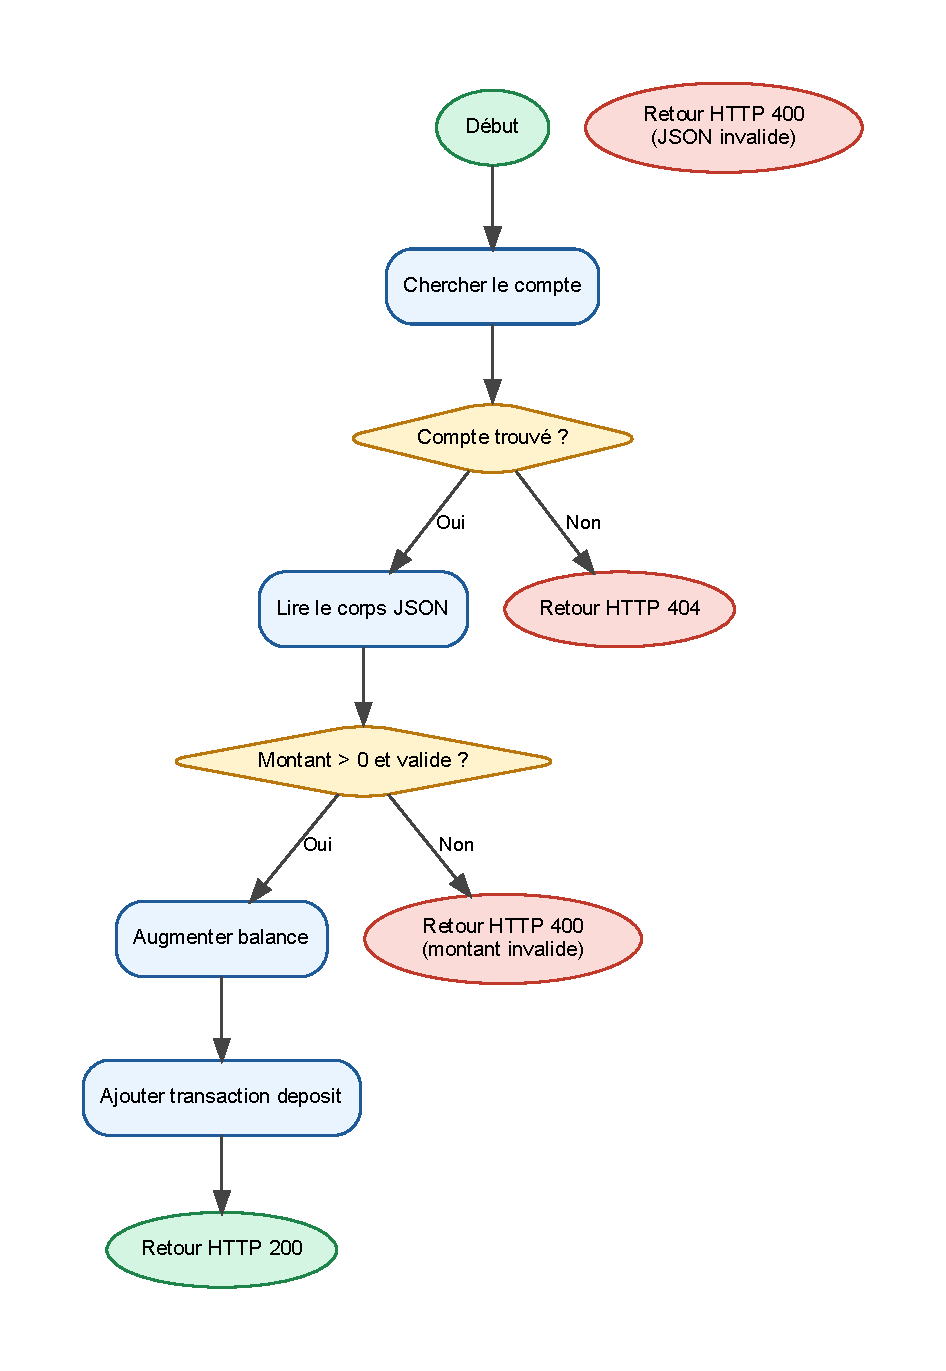
\includegraphics[width=0.74\textwidth]{docs/graphs/deposit.pdf}
\caption{Graphe de flot de contrôle du dépôt}
\end{figure}

\textbf{Chemins principaux}
\begin{itemize}[leftmargin=1cm]
    \item P1 : compte introuvable \(\rightarrow\) HTTP 404.
    \item P2 : montant invalide ou nul \(\rightarrow\) HTTP 400.
    \item P3 : dépôt valide \(\rightarrow\) solde augmenté et transaction enregistrée.
\end{itemize}

\subsection{Effectuer un retrait}

\begin{figure}[H]
\centering
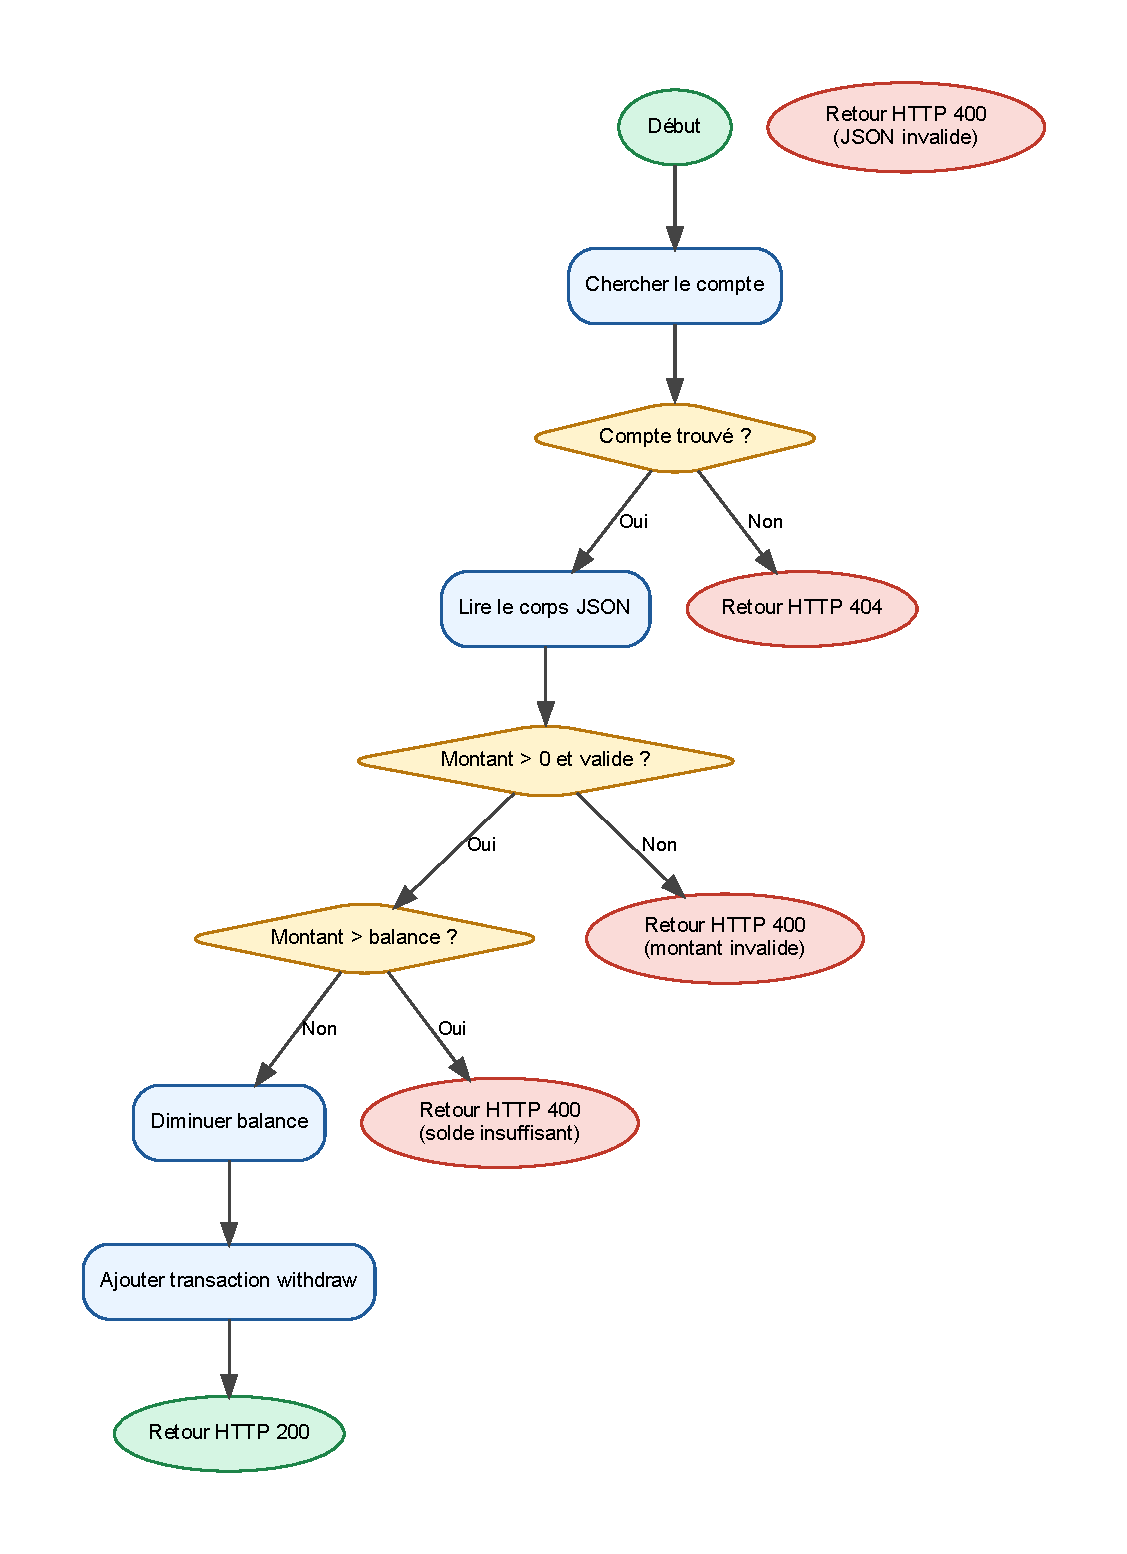
\includegraphics[width=0.78\textwidth]{docs/graphs/withdraw.pdf}
\caption{Graphe de flot de contrôle du retrait}
\end{figure}

\textbf{Chemins principaux}
\begin{itemize}[leftmargin=1cm]
    \item P1 : compte introuvable \(\rightarrow\) HTTP 404.
    \item P2 : montant invalide \(\rightarrow\) HTTP 400.
    \item P3 : solde insuffisant \(\rightarrow\) HTTP 400.
    \item P4 : retrait valide \(\rightarrow\) solde diminué et transaction enregistrée.
\end{itemize}

\section{Table de progression de couverture}

\begin{longtable}{|P{4.3cm}|P{4.2cm}|P{4.2cm}|P{3cm}|}
\hline
\rowcolor{lightgray}
\textbf{Fonction} & \textbf{Tests minimaux pour C1} & \textbf{Tests minimaux pour C2} & \textbf{Résultat} \\
\hline
Créer un compte & création sans solde + création avec solde + erreur champs + erreur solde négatif & idem & C1/C2 atteints \\
\hline
Lister les comptes & appel simple GET & appel simple GET & C1 atteint \\
\hline
Consulter un compte & compte existant + compte introuvable & idem & C1/C2 atteints \\
\hline
Effectuer un dépôt & dépôt valide + montant invalide + compte introuvable & idem & C1/C2 atteints \\
\hline
Effectuer un retrait & retrait valide + montant invalide + solde insuffisant + compte introuvable & idem & C1/C2 atteints \\
\hline
\end{longtable}

\section{Conclusion}

Cette analyse montre que les fonctions de dépôt et surtout de retrait contiennent plusieurs décisions importantes pour les tests structurels. Le retrait est plus complexe parce qu'il faut vérifier l'existence du compte, la validité du montant et la suffisance du solde.

Grâce aux graphes visuels et à la complexité cyclomatique, on peut déterminer clairement les chemins indépendants à couvrir et justifier les cas de test nécessaires pour les critères C1 et C2.

\end{document}
